\documentclass[main]{subfiles}

\begin{document}
	\begin{Reminder}
		\[f: U \to \R^m, \q a \in U, \q f \text{ --- диф. в т. } a \Ra\]
		\[U \subset \R^n\]
		\[\Mat(d_af) = \begin{pmatrix}
				\frac{\partial f_1}{\partial x_1}(a) & ...    & \frac{\partial f_1}{\partial x_n} (a) \\
				\vdots                               & \ddots & \vdots                                \\
				\frac{\partial f_m}{\partial x_1}(a) & ...    & \frac{\partial f_m}{\partial x_n} (a)
			\end{pmatrix}\]
		Якобиан - определитель матр. Якоби
	\end{Reminder}

	\begin{Example}
		\[f_1(\rho, \varphi),\q f_2(\rho, \varphi)\]
		\[f(\rho, \varphi) = (\rho \cos \varphi; \rho \sin \varphi)\]
		\[f: [0, +\infty) \times \R \to \R^2\]
		\[J = d_{(\rho , \varphi)}f = \begin{pmatrix}
				\cos \varphi & -\rho \sin \varphi\\
				\sin \varphi & \rho \cos \varphi
			\end{pmatrix} \]
		\[\det(J) = \rho\]
	\end{Example}

	\begin{remark}
		Но из существования частной произв. (в общ. случ.) не следует диф-ть!
	\end{remark}

	\begin{examples}
		1)
		\[f(x, y) = \begin{cases}
				\frac{x^2 y}{x^2 + y^2}, & (x, y) \neq 0 \\
				0,                       & (x, y) = 0
			\end{cases}\]
		Частн. пр-ые в т. $(0, 0)$
		\[f_x' = \lim_{\triangle x \to 0} \frac{f(\triangle x, 0) - f(0, 0)}{\triangle x} = 0 \]
		\[f_y' = \lim_{\triangle y \to 0} \frac{f(0, \triangle y) - f(0, 0)}{\triangle y} = 0\]
		\begin{figure}[H]
			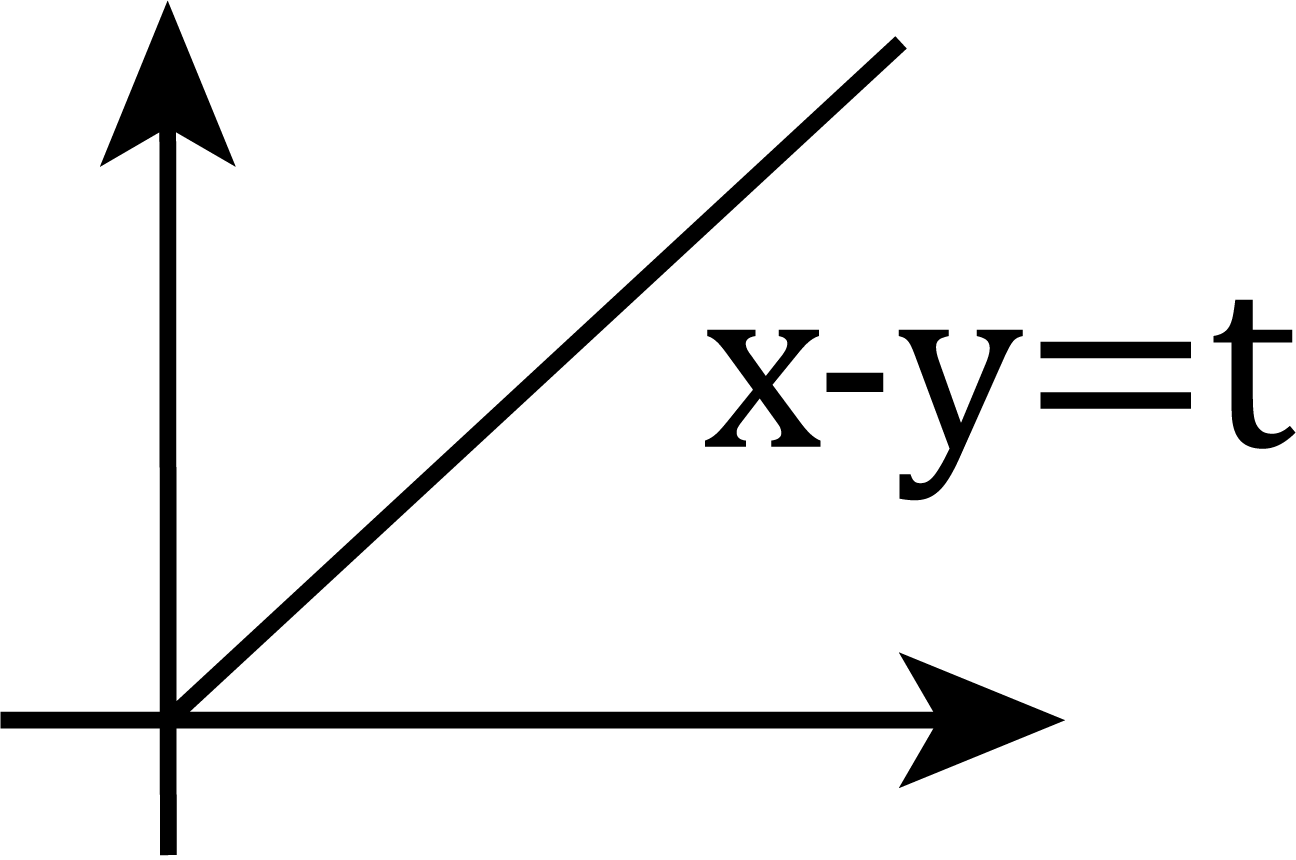
\includegraphics[width = 2.5cm]{pics/4_1}
			\centering
		\end{figure}
		Если бы f --- диф. в т. $(0, 0)$, то
		\[f(x, y) = f(0, 0) + (0, 0) \begin{pmatrix}
				x \\
				y
			\end{pmatrix}
			+ o(\sqrt{x^2 + y^2})
		\]
		\[\lim_{(x, y) \to (0, 0)} \frac{||f(x, y) - f(0, 0) - (0, 0) \begin{pmatrix}
					x \\
					y
				\end{pmatrix}||}{\sqrt{x^2 + y^2}} =
			\lim_{(x, y) \to (0, 0)} \frac{x^2|y|}{ \sqrt{x^2 + y^2}^3} \]
		\[\text{При } (x, y) = (t, t)\]
		\[\frac{x^2|y|}{\sqrt{x^2 + y^2}} \to \frac{1}{2\sqrt{2}} \neq 0\]
		2)
		\[f(x, y) = \begin{cases}
				\frac{x^2 y}{x^4 y^2} & (x, y) \neq (0, 0) \\
				0 , (x, y) = (0, 0)
			\end{cases}\]
		частн. произв. $\exists$ во всех т., но $f$ разрывна в $(0, 0)$\\
		3)
		\[f: \R^2 \to \R^2\]
		\[f(x_1, x_2) = \begin{pmatrix}
				x_1 \cdot x_2 \\
				x_1 + 2x_2
			\end{pmatrix}\]
		\[a = (1, -1)\]
		\[\frac{\partial f_1}{\partial x_1} = x_2 \q\q \frac{\partial f_1}{\partial x_2} = x_1\]
		\[\frac{\partial f_2}{\partial x_1} = 1 \q\q \frac{\partial f_2}{\partial x_2} = 2\]
		\[\text{Mat}(d_a f) = \begin{pmatrix}
				-1 & 1 \\
				1  & 2
			\end{pmatrix}\]
		\[h = \begin{pmatrix}
				0 & 2 \\
				0 & 3
			\end{pmatrix} \text{ --- приращение}\]
		\[d_a f(h) = \begin{pmatrix}
				-1 & 1 \\
				1  & 2
			\end{pmatrix}
			\begin{pmatrix}
				0 & 2 \\
				0 & 3
			\end{pmatrix} =
			\begin{pmatrix}
				0 & 1 \\
				0 & 8
			\end{pmatrix}\]
		\[f(a + h) = f(a) + d_af(h) + o(||h||)\]
	\end{examples}

	\begin{Definition}
		\[f : U \to \R^1 \q U \subset \R^n, \q f \text{ --- диф. в } a \]
		\[d_a f \in \LL(\R^n, \R^1) \text{ --- лин. ф}\]
		\[\text{Mat}(d_af) = (\frac{\partial f}{\partial x_1}; \frac{\partial f}{\partial x_2} ...
			\frac{\partial f}{\partial x_n})(a)\]
		$\nabla \text{ -- "набла"{} }$\\
		Градиент $f$ в т. a (f диф в т. a)
		\[\text{grad}_a f = \nabla_a f = (\frac{\partial f}{\partial x_1}, \frac{\partial f}{\partial x_2}, ...,
			\frac{\partial f}{\partial x_n})(a)\]
		\[d_af(h) = (\nabla_a f; h) = \sum^{n}_{k = 1} \frac{\partial f}{\partial x_k} \cdot h_k \]
	\end{Definition}

	\newpage
	\subsection{Теорема о дифференцировании композиции}

	\begin{Theorem}[диф-ние композиции]
		\[f: U \to \R^m; \q U \subset \R^n \q\q f(U) \subset V \subset \R^m\]
		\[g: V \to \R^k \q\q\q\q\q U, V \text{ - откр.}\]
		\[f \text{ --- диф. в т. } a \in U\]
		\[g \text{ --- диф. в т. } f(a) = b\]
		\[\text{Тогда } h = g \circ f \text{ --- диф. в т. } a, \text{ причем }\]
		\[d_ah = d_{f(a)}g \circ d_{a} f \in \LL(\R^n, \R^k)\]
	\end{Theorem}

	\begin{Proof}
		\[A = d_a f; \q B = d_b g \q\q f(x) := f(a) + A(x - a) + o||x - a|| \q x \to  a\]
		\[r_f(x) = f(x) - f(a) - A(x - a) = o|| x - a|| \q (x \to a)\]
		\[r_g(y) = g(y) - g(b) - B(y - b) = o|| y - b|| \q (y \to b)\]
		\[r_h(x) := h(x) - h(a) - BA(x-a) \os{?}{=} o||x-a|| \q (x \to a)\]
		\[g(f(a)) = h(a)\]
		Хотим показать, что
		\[r_h(x) = o(||x-a||) \q x \to  a\]
		\[r_h(x) =\ub{ = r_g(f(x))}{ g(f(x)) - g(b) - B(f(x) - b)} + B(f(x) - b) - BA(x-a) = \]
		\[=r_g(f(x)) + B(\ub{=r_f(x)}{f(x) - f(a) - A(x-a))}\]
		\[r_h(x) = r_g(f(x)) + B(r_f(x))\q\q\q ||Ax|| \leq ||A|| \cdot ||x||\]
		\[||r_h(x)|| \leq ||r_g(f(x))|| + ||B|| \cdot ||r_f(x)|| \]
		\[\text{Пусть } \mathcal{E} > 0\]
		\begin{enumerate}
			\item (из диф-ти g) $\exists \delta > 0 :$
			      \[\forall y: ||y-b|| < \delta \RA ||r_g(y)|| < \mathcal{E} \cdot ||y - b||\]
			\item $\exists \alpha : $
			      \begin{enumerate}
				      \item (из диф-сти f в т. a)
				            \[||r_f(x) || < \mathcal{E}||x - a|| \q \forall x : ||x - a|| < \alpha\]
				      \item $\forall x : ||x - a|| < \alpha$
				            \[||f(x) - f(a)|| < \delta \text{ (т.к. f непр в т. a) } \q\q f(a) = b\]
			      \end{enumerate}
		\end{enumerate}
		\[\text{Возьмем } x : ||x-a|| < \alpha\]
		\[\os{ 2\text{б} }{\Ra}
			||f(x) - b|| < \delta \os{(1)}{\Ra}
			||r_g(f(x))|| < \mathcal{E} \cdot||f(x) - b||\]
		\[||f(x) - b|| = ||r_f(x) + A(x-a)|| \leq ||r_f(x)|| + ||A|| \cdot ||x - a|| \os{2a}{<}\]
		\[< \mathcal{E} \cdot ||x - a|| + ||A|| \cdot ||x - a||\]
		\[||r_h(x)|| \leq || r_g(f(x))|| + ||B|| \cdot ||r_f(x)|| <\]
		\[\mathcal{E}(\mathcal{E} ||x-a|| + ||A|| \cdot ||x-a||) + ||B|| \cdot \mathcal{E} ||x-a|| = \]
		\[= (\mathcal{E}^2 + ||A|| \mathcal{E} + ||B|| \mathcal{E}) \cdot ||x-a||\]
		Выполняется определение $\ol{o}$
	\end{Proof}

	\newpage
	\subsection{Частные производные композиции. Дифференциал скалярного произведения}

	\begin{Consequence}[1]
		\[\frac{\partial (g \circ f)_l}{\partial x_j} =
			\sum^m_{i = 1} \frac{\partial g_l}{\partial y_i}(b) \frac{\partial f_i}{\partial x_j}(a) \]
		\[d_a g \circ f = d_{f(a)}g \circ d_a f \q\q \text{комп.} \leftrightarrow \text{пр-ие матриц} \]
		\[\begin{pmatrix}
				\frac{\partial g_1}{\partial y_1} & ... & \frac{\partial g_1}{\partial y_m} \\
				...                                                                         \\
				\frac{\partial g_k}{\partial y_1} & ... & \frac{\partial g_k}{\partial g_m}
			\end{pmatrix}
			\begin{pmatrix}
				\frac{\partial f_1}{\partial x_1} & ... & \frac{\partial f_1}{\partial x_n} \\
				...                                                                         \\
				\frac{\partial f_m}{\partial x_1} & ... & \frac{\partial f_m}{\partial x_n}
			\end{pmatrix}
		\]
	\end{Consequence}

	\begin{Consequence}[2]
		\[U \subset \R^n,\q f,\ g : U \to  \R \text{ --- диф. в т. a}\]
		\[\text{Тогда } d_a(f \cdot g) = f(a) \cdot d_a g + g(a) \cdot d_af\]
	\end{Consequence}

	\begin{proof}
		\begin{enumerate}
			\item Пусть $f = g \q d_a f^2$
			      \[\varphi(t) = t^2 \q\q d_t \varphi(h) = 2t \cdot h\]
			      \[d_a f^2 = d_a \varphi \circ f = d_{f(a)}  \varphi \circ d_{a} f = 2f(a) \cdot d_a f\]
			\item $d_a(f \cdot g) = d_a (\frac{1}{4}[(f+g)^2 - (f-g)^2]) = $
			      \[= \frac{1}{4} [2 (f(a) + g(a)) d_a (f+g) - 2(f(a) - g(a))d_a(f - g)]= \]
			      \[= f(a) d_a g + g(a) d_a f\]
		\end{enumerate}
	\end{proof}

	\begin{Consequence} [3]
		\[f, g : U \to  \R^n, \q U \subset \R^m\]
		\[f, g \text{ --- диф. в т. } a \in U\]
		\[(f; g) \text{ - ск. пр-ие}\]
		\[\text{Тогда } d_a(f, g) = (f(a); d_a g) + (d_a f; g(a))\]
	\end{Consequence}

	\newpage
	\subsection{Градиент, его свойства}

	Вернемся к градиенту
	\[f : U \to \R^1 \q U \subset \R^n \q\q f \text{ --- диф. в т. a} \in U \]
	\[d_a f(h) = (\nabla_a f; h)\]
	\[\nabla_a f = (\frac{\partial f}{\partial x_1}(a), ..., \frac{\partial f}{\partial x_n}(a))\]

	\begin{properties}[геометрич. св-ва градиента]
		\begin{enumerate}
			\item $f$ возрастает в напр. h в т. a, если $(\nabla_a f; h) > 0$\\
			      и убывает, если $(\nabla_a f; h) < 0$
			      \begin{figure}[h!]
				      \center{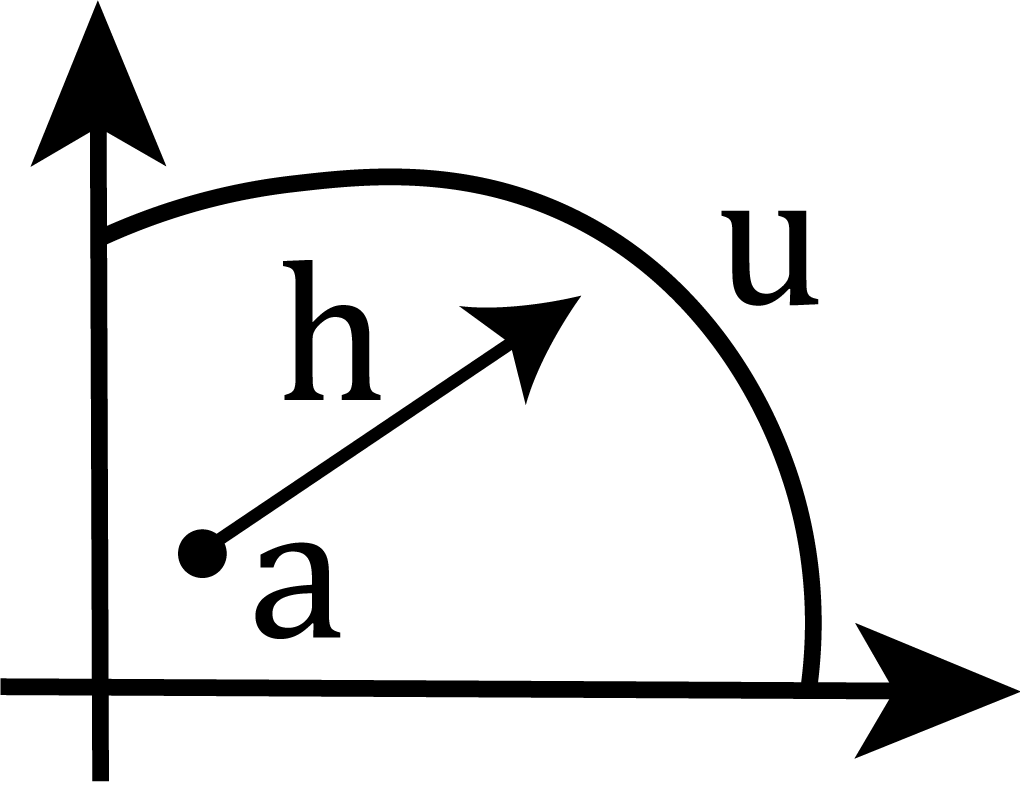
\includegraphics[width = 2.5cm]{pics/4_2}}
			      \end{figure}
				  Пусть $||h||=1$
			      \[f(a + t \cdot h) = f(a) + \us{> 0 \text{ (угол острый, $\cos > 0$)}}{(\nabla_a f; th)} + o(||th||) \q\q o(||th||) = o(||t||)\]
			      \[\text{Пусть } t > 0\]
			      \[\frac{f(a + th) - f(a)}{t} = \ub{>0}{\frac{t \cdot (\nabla_a f, h)}{t}} + \ub{\ra 0}{\frac{o(t)}{t}} > 0\]
			      \[ \text{Начиная с нек. места }(\forall\ 0 < t < \delta)\]
			      \[\os{0 < t < \delta}{\Ra} f(a + th) > f(a)\]
			\item (экстремальное св-во градиента)\\
			      Если $\nabla_af \neq 0$, то направление наибольшего возрастания f \\
			      совпадает с направлением градиента
			      \[||e|| = 1\]
			      \[|\frac{\partial f}{\partial e}(a)| = |d_af(e)| = |(\vec{\nabla}_af; \vec{e})| \leq || \nabla_a f|| \cdot \us{=1}{||e||} = ||\nabla_a f||\]
			      Если $e = \frac{\nabla_a f}{|| \nabla_a f||} \text{ то } |\frac{\partial f}{\partial e}(a)| =
				      ||\nabla_a f||$
			\item $f : U \to \R$ \q f --- диф в т. $a \in U$ \q\q $U \subset \R^n$\\
			      Если a --- т. локального экстремума f $\Ra$
			      \[\vec{\nabla_a} f = \vec{0}\]
			\item Пусть $\Gamma_a = \{x \in U: f(x) = f(a)\}$\\
			      \[\text{Тогда } \nabla_af \perp \Gamma_a\]
			      \[\text{Т.е. } \forall \text{ Гладкой кривой } \q \gamma: [-1, 1] \to \Gamma_a, \]
			      \[\text{проход. через т. a} \q\q (\gamma(0) = a)\]
			      \[\gamma(t)' = \begin{pmatrix}
					      \gamma_1'(t) \\
					      \vdots       \\
					      \gamma_n'(t)
				      \end{pmatrix} \text{ --- касат. вектор к } \Gamma_a \text{ в т. a}\]
			      \[\text{Говорят, что } \vec{v} \text{ --- ортог. } \Gamma_a \text{ в т. a}\]
			      \[\text{Если } \vec{v} \perp \gamma'(0) \q \forall \text{ гладкой кривой } \gamma : \gamma(0) = a\]
		\end{enumerate}
	\end{properties}

	\begin{Example}
		\[f(x, y, z) = x^2 + y^2 + z^2\]
		\[\nabla_{(x, y, z)} f = (2x; 2y; 2z) = 2(x, y, z)\]
		\begin{figure}[h!]
			\center{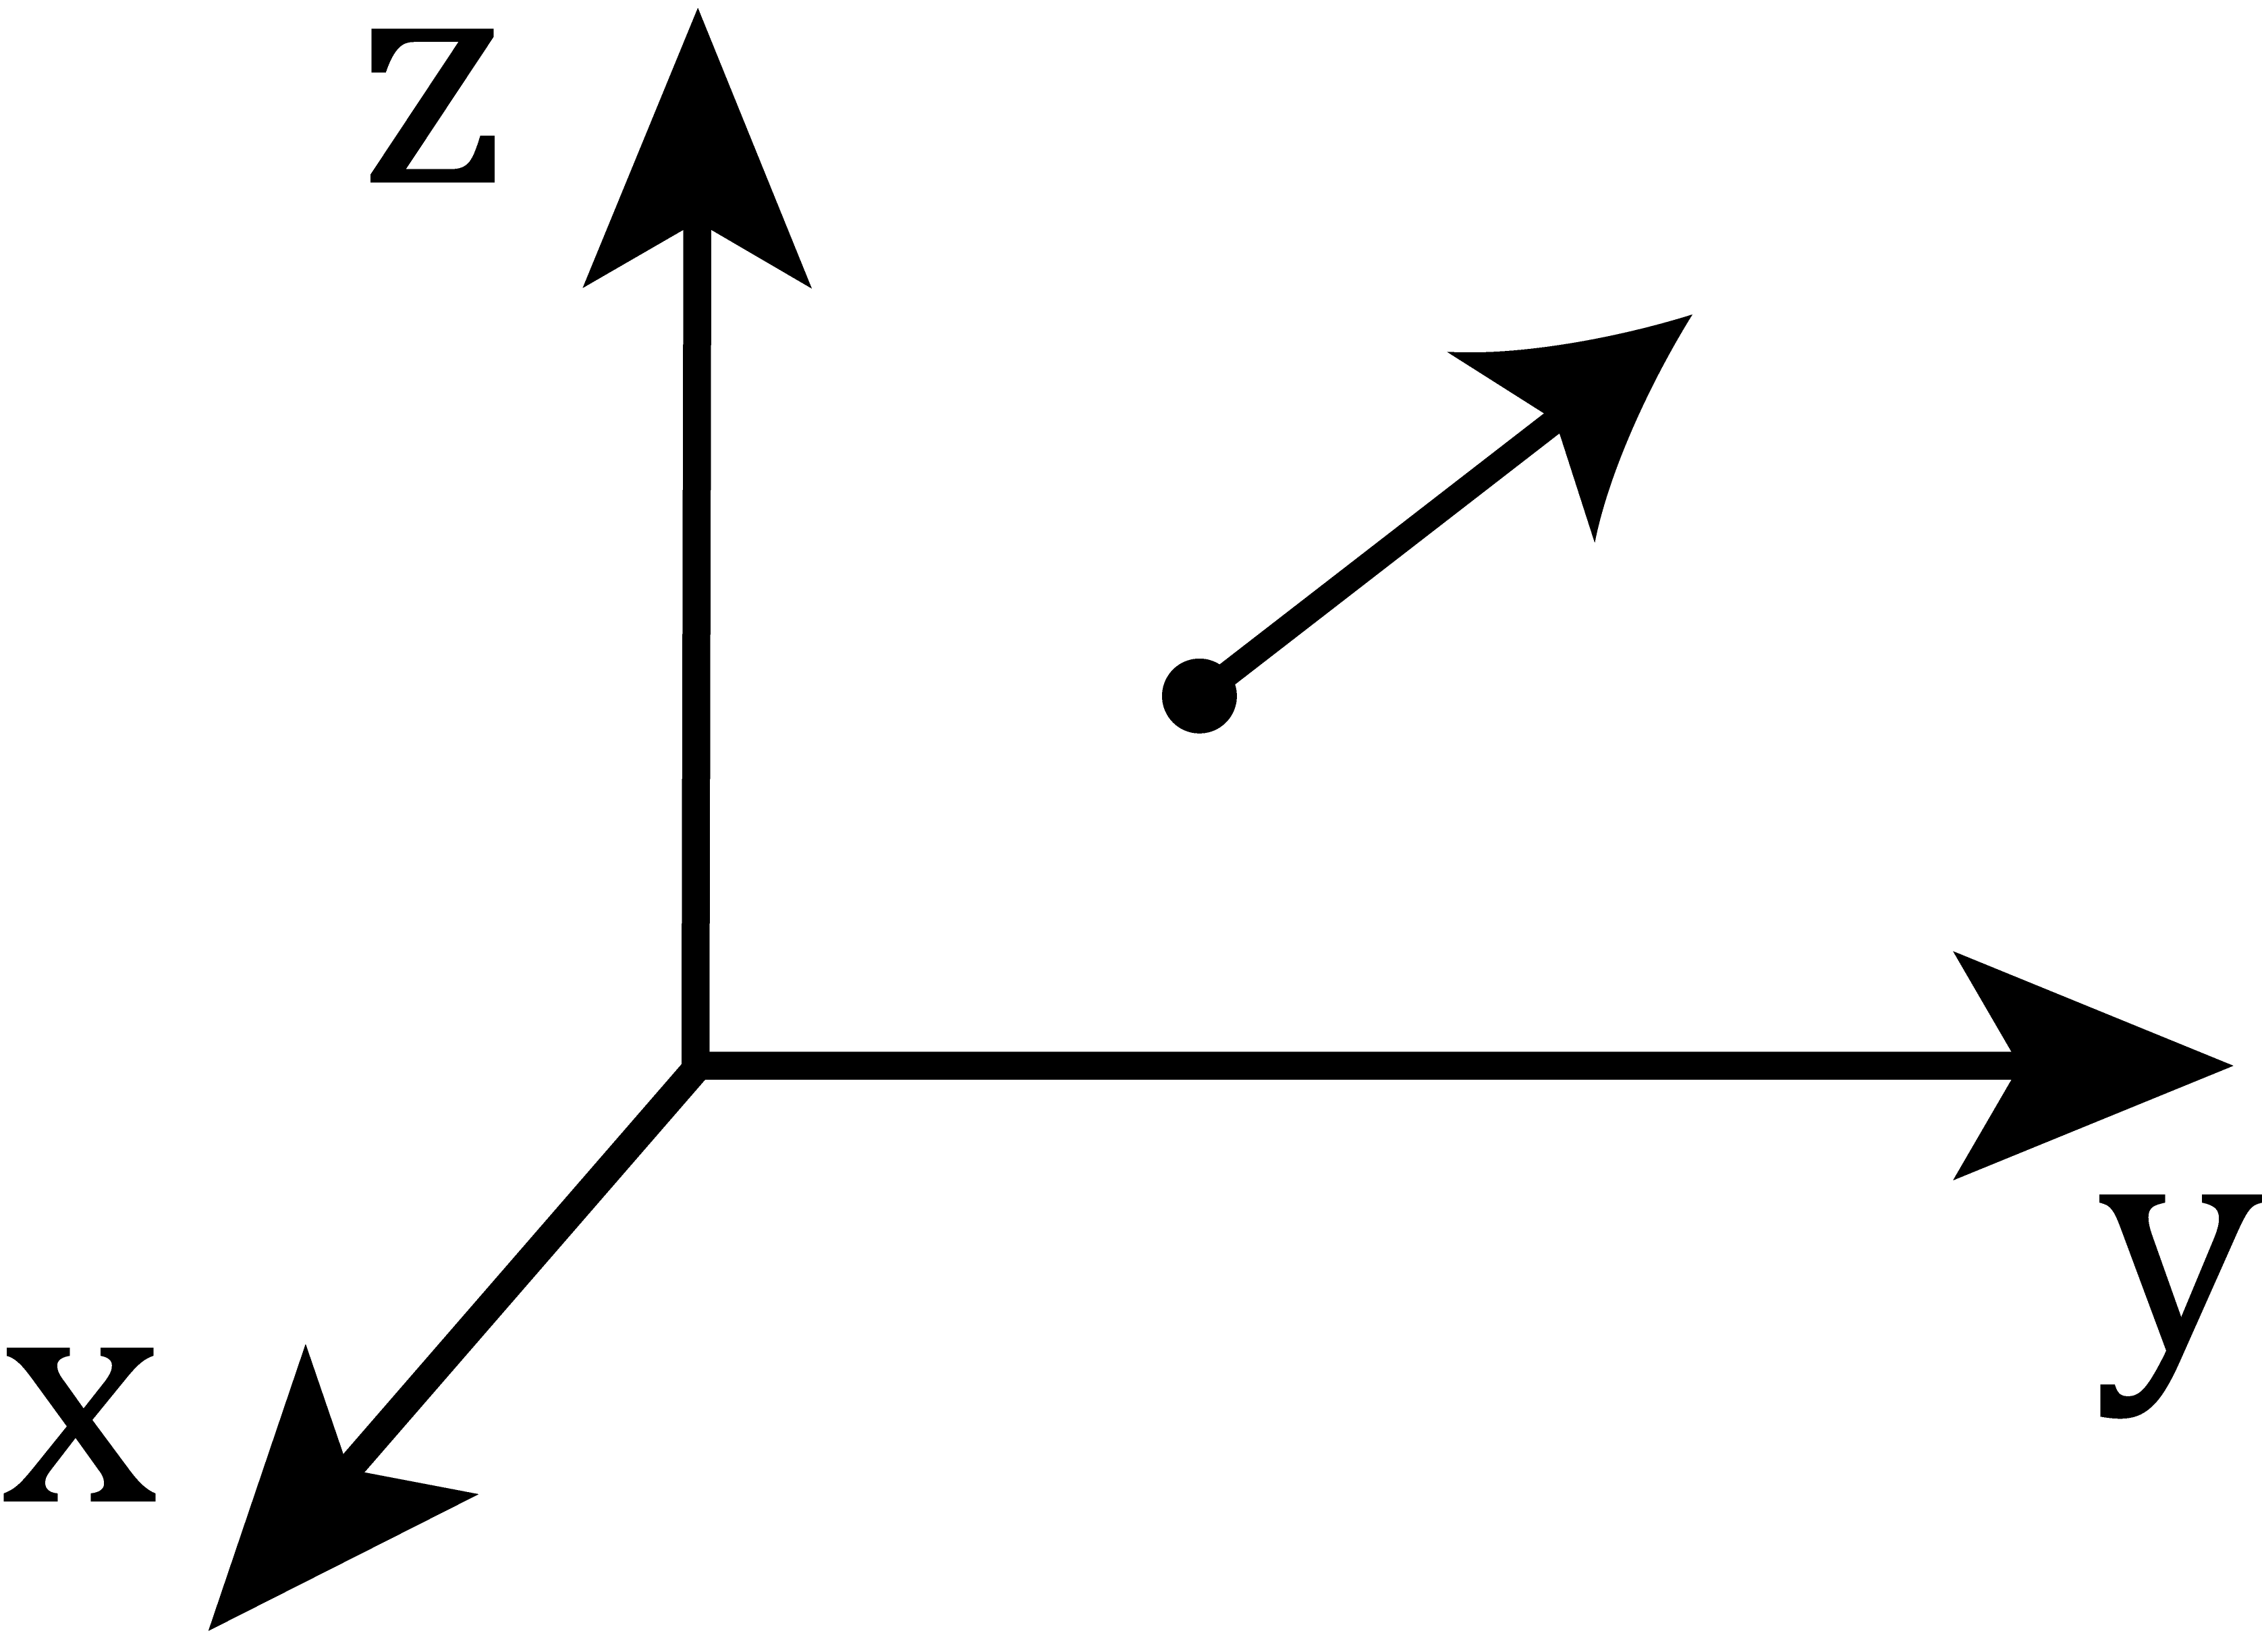
\includegraphics[width = 2.5cm]{pics/4_3}}
		\end{figure}
	\end{Example}

	\begin{Definition}
		\[f: U \to \R; \q a \in U \text{ --- т. лок. макс. (минимума)}\]
		\[\text{Если } \exists V_a : \forall x \in V_a\]
		\[f(x) \leq f(a) \q (f(x) \geq f(a))\]
	\end{Definition}

	\begin{Example}[к свойствам]
		\[f(x, y, z) = x^2 + y^2 + z^2\]
		\[a(1, 1, 1)\]
		\[\Gamma_a = \{(x, y, z): x^2 + y^2 + z ^2 = 3\}\]
		\[\nabla_a f = 2(a_1, a_2, a_3) = (2, 2, 2)\]
		\begin{figure}[h!]
			\center{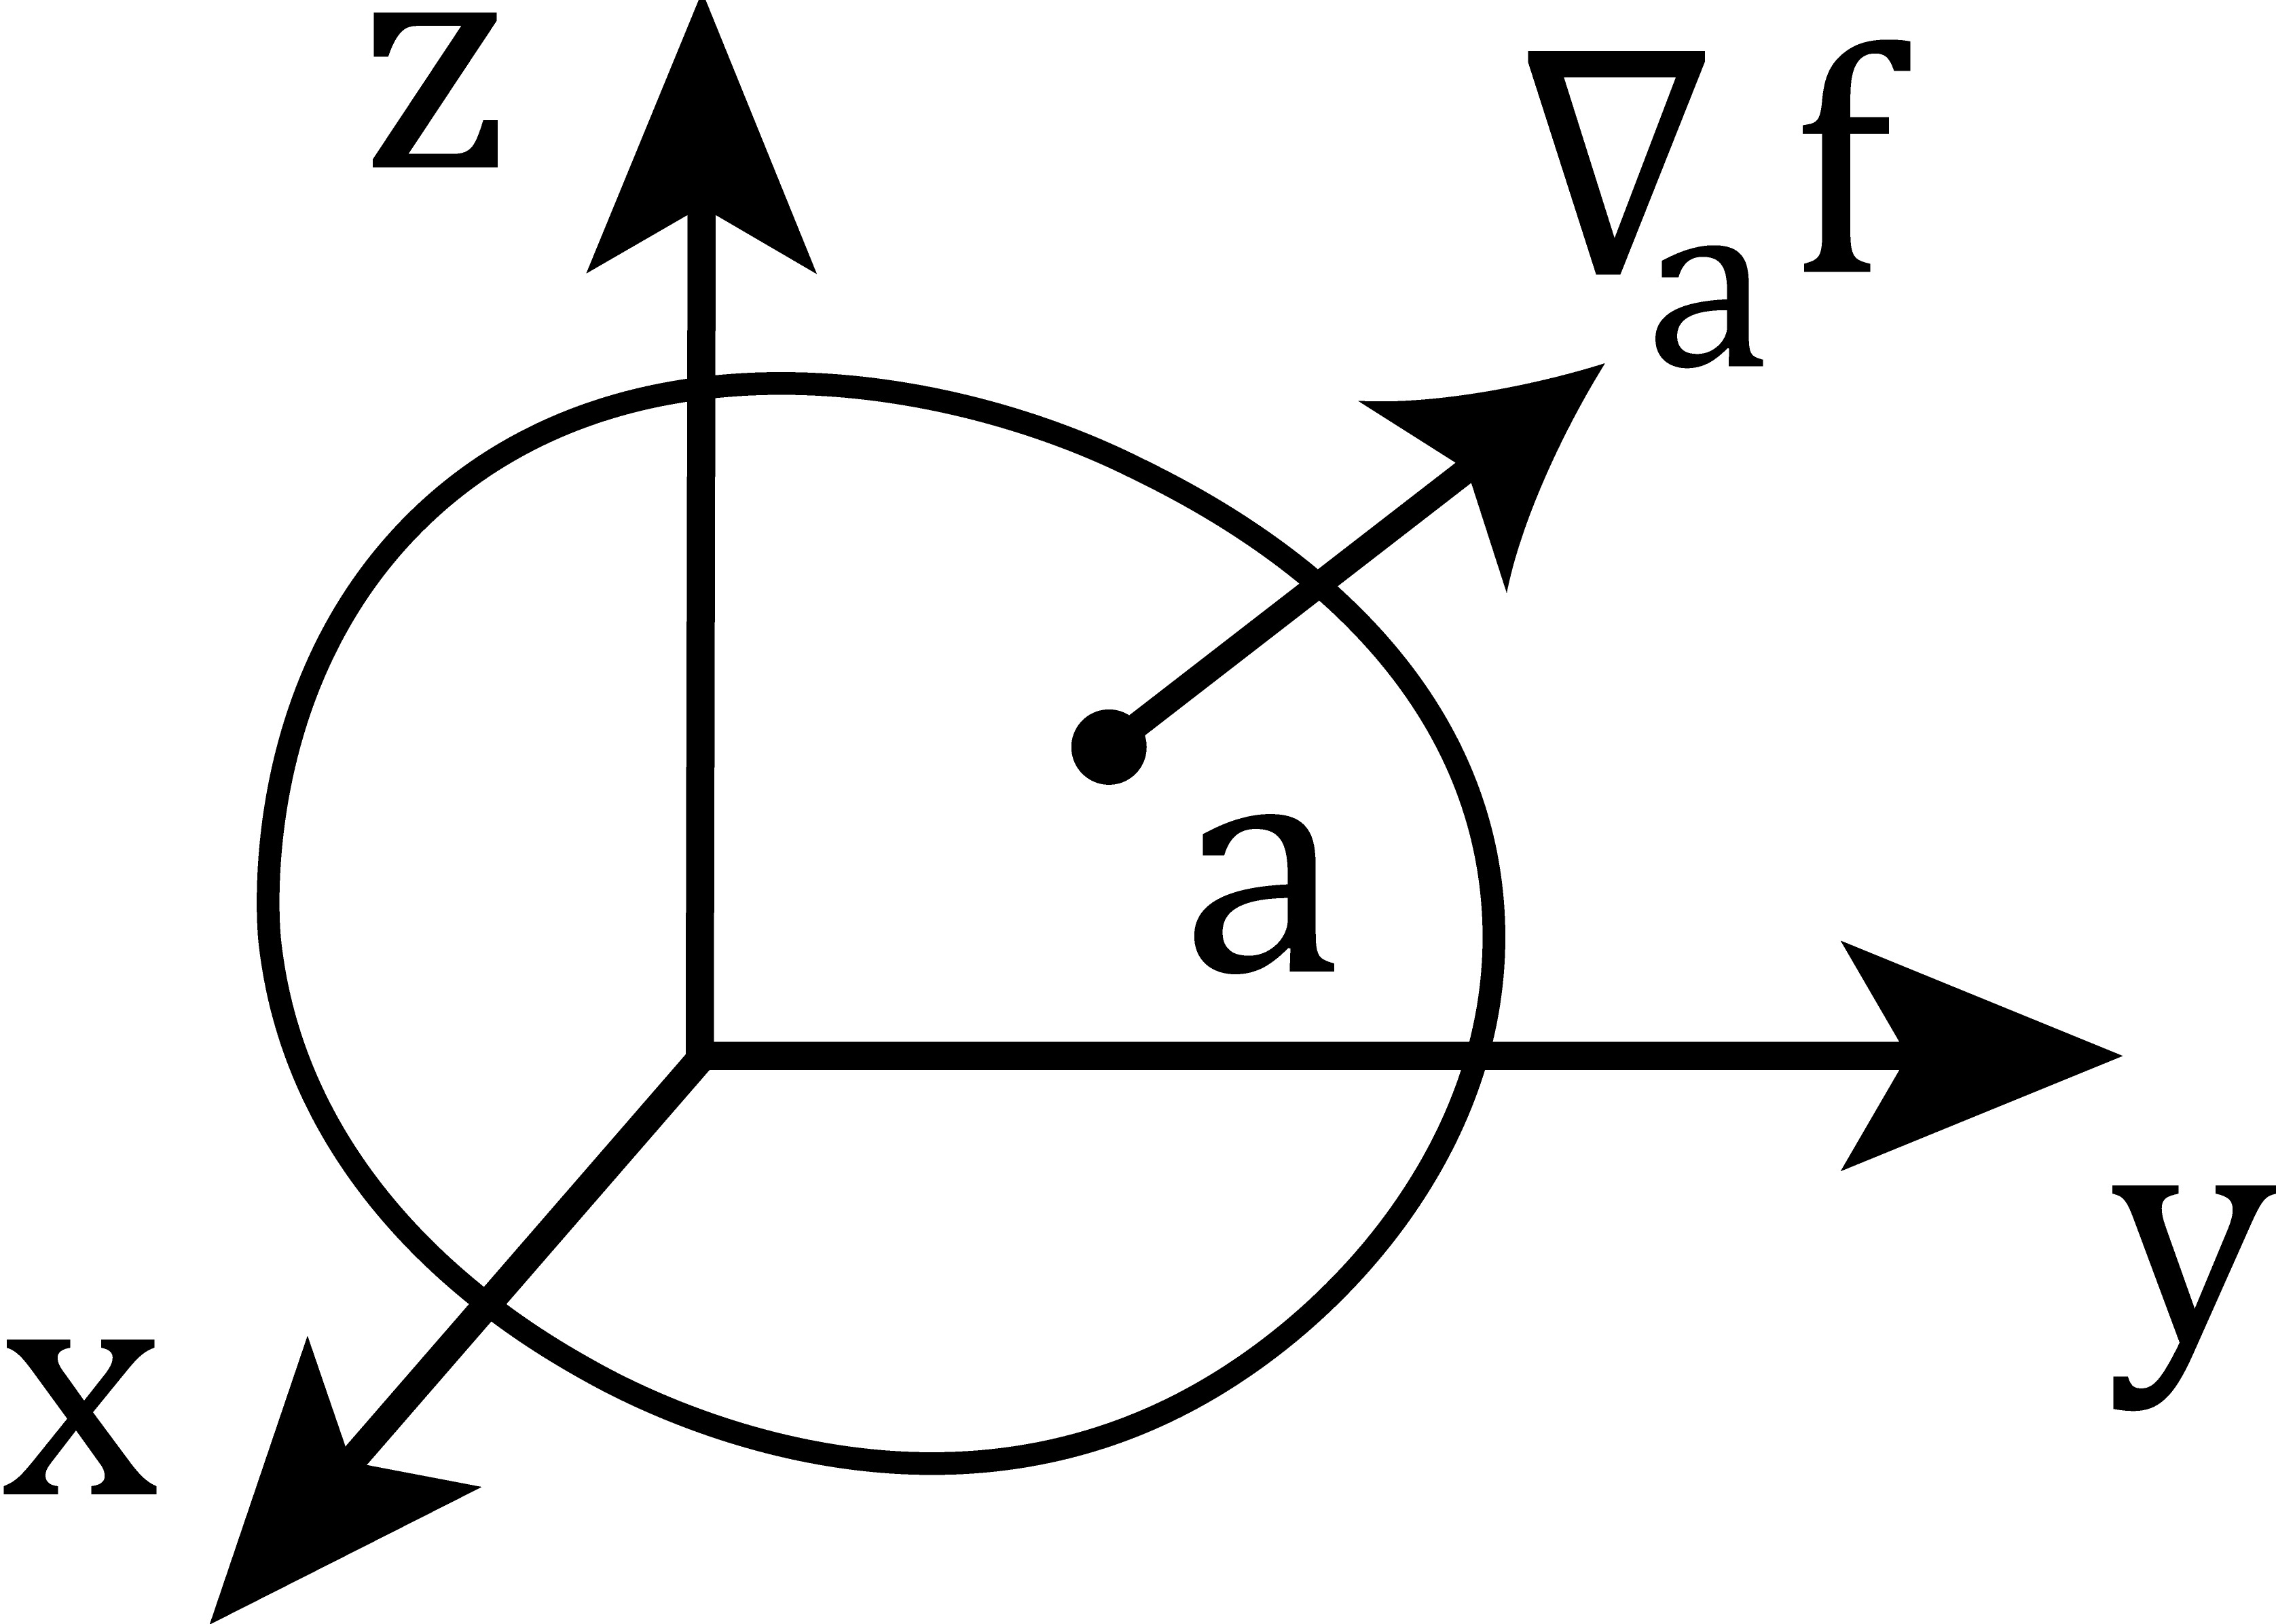
\includegraphics[width = 3cm]{pics/4_5}}
		\end{figure}
	\end{Example}

	\begin{Proof}
		\[\Gamma_a = \{x \in U \q f(x) = f(a)\}\]
		\[\gamma: [-1, 1] \to \Gamma_a \q \gamma(0) = a\]
		\[\us{\text{обычная ф-я 1 перем.}}{f(\gamma(t))} = f(a) \q \forall t \in [-1, 1]\]
		\[0 = d_0(f(\gamma(t))) = d_{\gamma(0)} f \circ d_0\gamma = d_a f \circ \gamma'(0) = \]
		\[= \nabla_a f \cdot \gamma'(0) \Ra \nabla_a f \perp \gamma'(0)\]
	\end{Proof}

	\newpage
	\subsection{Дифференцируемость функции с непрерывными частными производными}

	\begin{Definition}
		\[f: U \to  \R^m \q U \subset \R^n \q a \in U\]
		\[f \text{ --- непр. диф в т. } a \text{, если:}\]
		\begin{enumerate}
			\item Все частные производные определены в некоторой\\ окрестности т. a
			\item Непр. в т. a
		\end{enumerate}
		Говорят, что f --- непр. диф. на U, если она непр. диф. в каждой точке
		\[f \in C^1(U)\]
	\end{Definition}

	\begin{Lemma} [т. о среднем]
		\[f : U \to  \R \q a \in U \subset \R^n, \q \text{все частные пр-е определены в } V_a \subset U\]
		\[\sqsupset h: a + h \in V_a\]
		\[\text{Тогда } \exists c^1, c^2, ..., c^k:\]
		\[f(a + h) - f(a) = \sum^n_{k = 1}  \frac{\partial f}{\partial x_k}(c^k) \cdot h_k\]
	\end{Lemma}

	\begin{Proof} \
		\begin{figure}[h!]
			\center{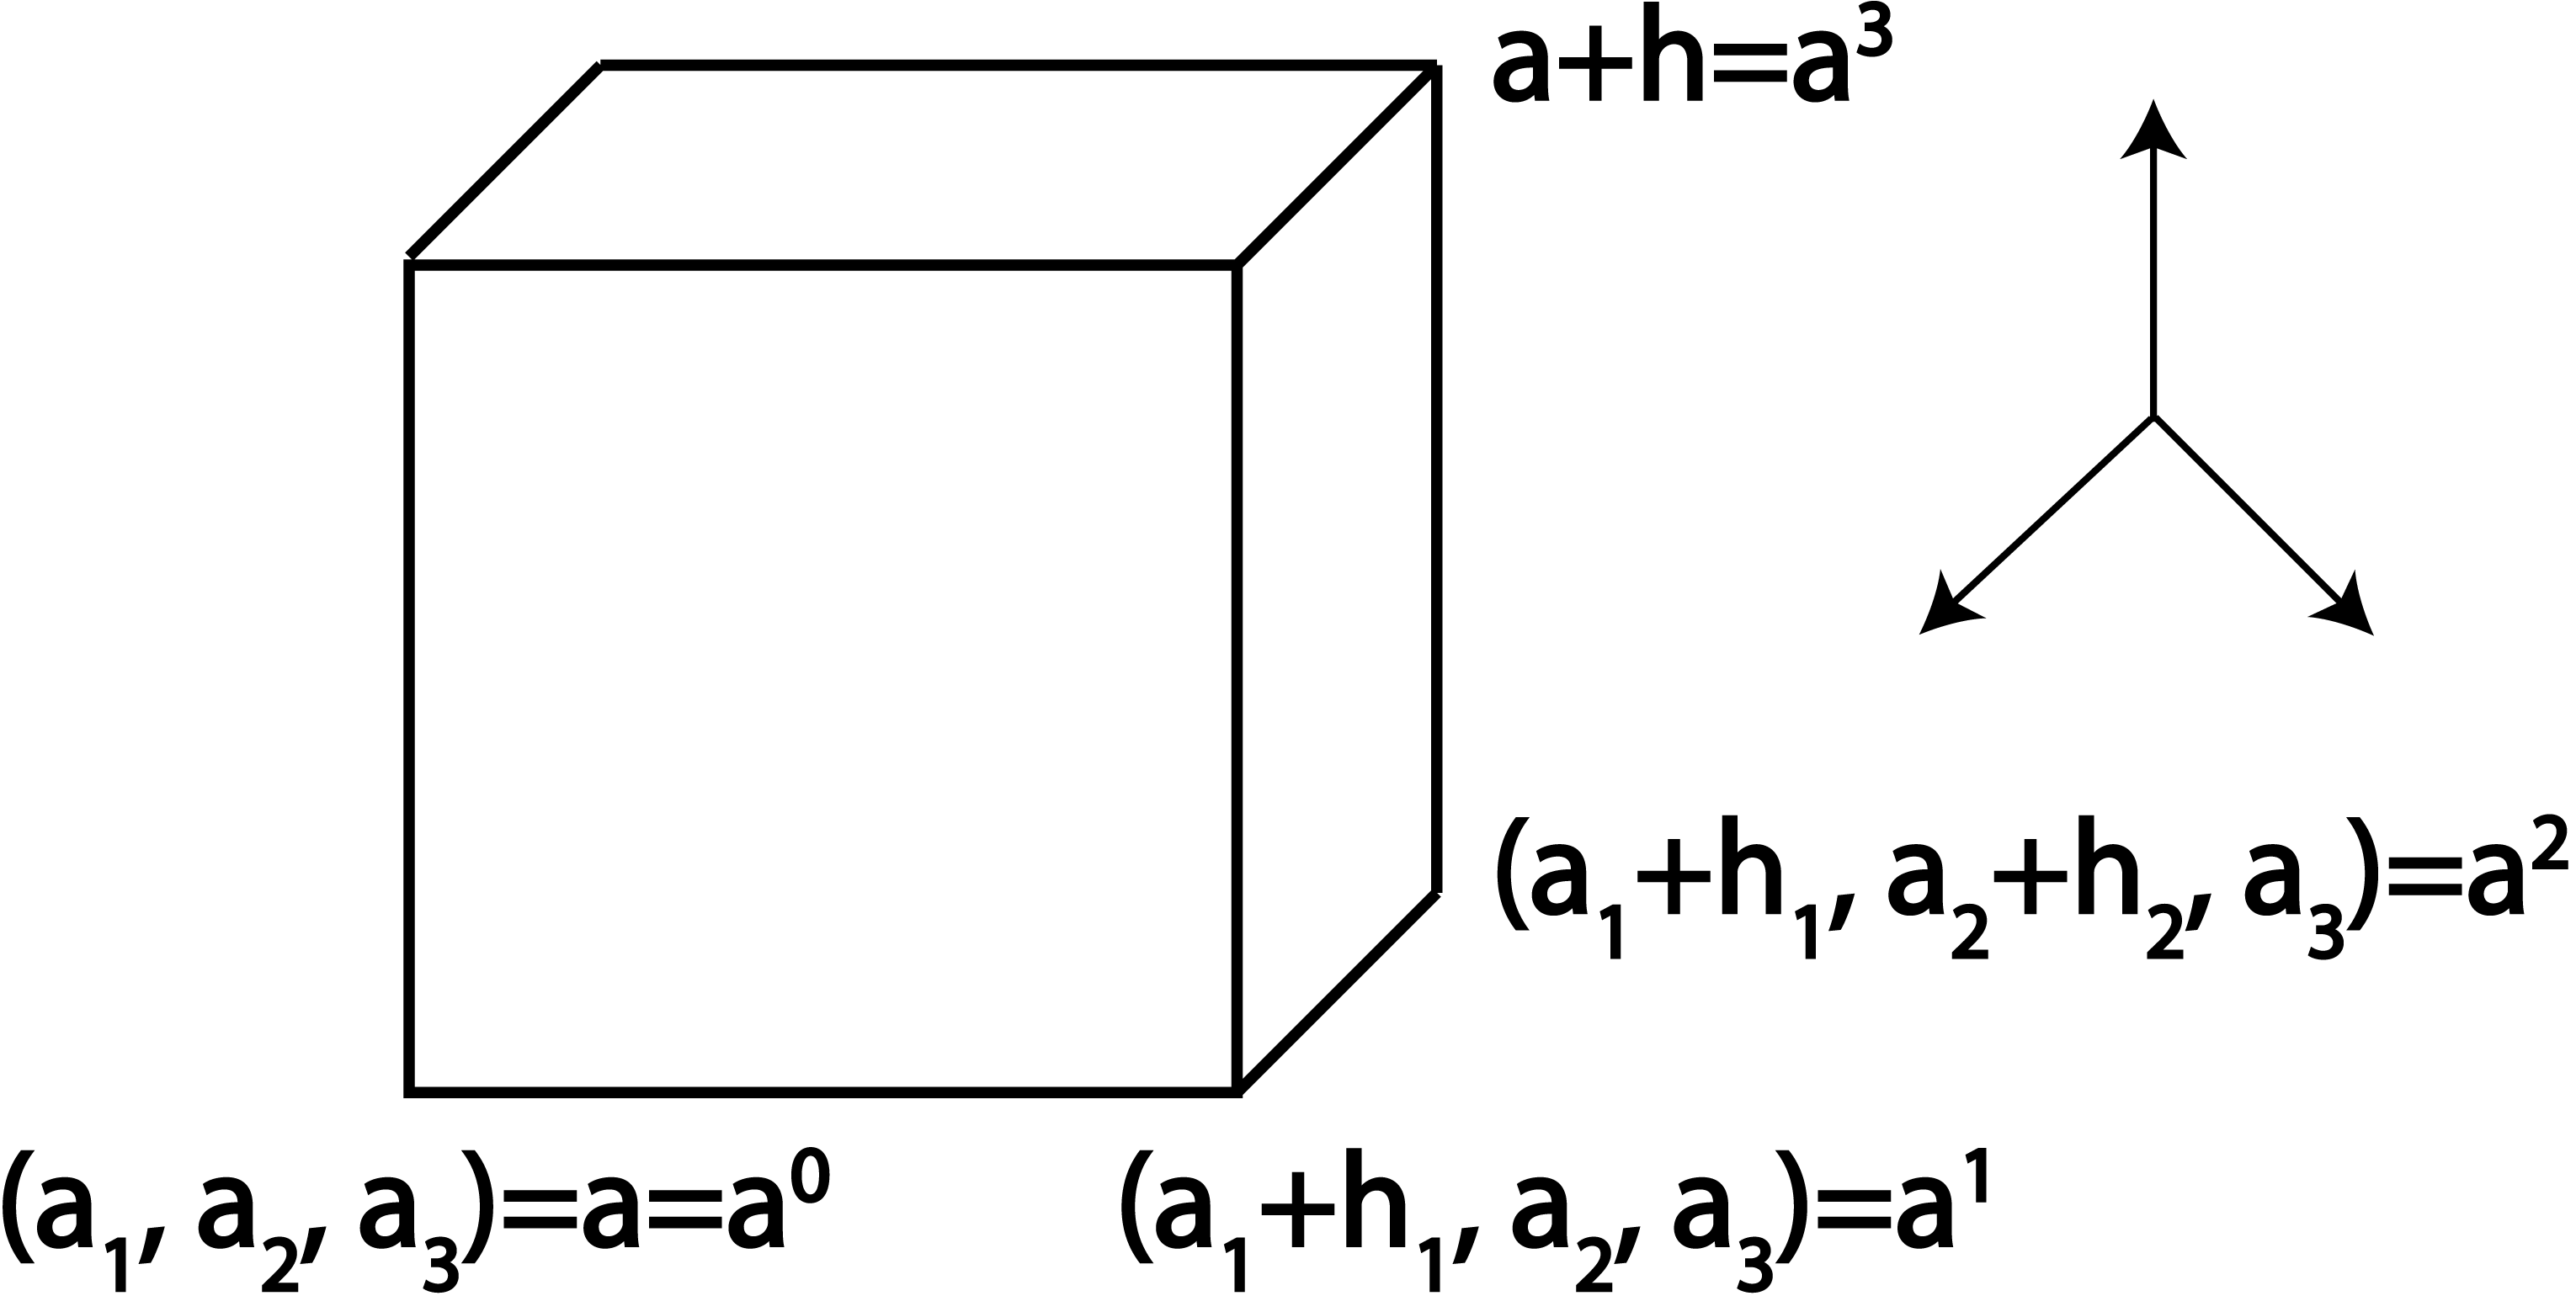
\includegraphics[width = 7cm]{pics/4_6}}
		\end{figure}
		\[F_k(t) = f(a^{k - 1} + t \cdot h_ke_k) \]
		\[a^{k-1} \text{ --- т. ребра } (a^{k-1}; a^k) \q\q o \leq t \leq 1 \]
		\[F'_k(t) = f'_{x_k} (\us{= a_1 + h_1,\ a_2 + h_2,\ ...,\ a_{k-1} + h_{k-1},\ a_k + t h_k,\ a_{k+1},\ ...,\ a_n}
			{a^{k - 1} + t \cdot h_k \cdot e_k}) \cdot h_k\]
		По т. Лагранжа $\exists \xi^k \in (0, 1) $
		\[F_k(1) - F_k(0) = F_k'(\xi^k)(1-0) = \frac{\partial f}{\partial x_k} (\us{= c_k}{a^{k - 1} + \xi^k h_k e_k}) \cdot h_k\]
		\[c^k \in V_a\]
		\[f(\us{ = a^n}{a + h}) - f(\us{=a^0}{a}) = \sum^n_{k = 1} f(a^k) - f(a^{k - 1}) =  \]
		\[= \sum_{k = 1}^n  F_k(1) - F_k(0) = \sum^n_{k = 1} \frac{\partial f}{\partial x_k} (c_k) h_k \]
	\end{Proof}
\end{document}
